For the results shown in Chapter~\ref{chap:HPROMResults}, all simulations have simply \textit{reconstructed} the training data. That is, the geometry, initial conditions, boundary conditions, and simulation duration of each PROM is identical to those of the FOM from which the training data is extracted. Although these simulations were successful in this effort, the ultimate goal of any data-driven method is \textit{generalizability}. To be truly useful for engineering applications, such methods must be able to make fast and accurate predictions for unseen configurations which are not accounted for in the training data. 

\section{Failure of Static Trial Bases}

The PROMs investigated in Chapter~\ref{chap:HPROMResults} are, unfortunately, not generalizable. To demonstrate this for the truncated CVRC case examined in Section~\ref{sec:cvrc}, the unsampled MP-LSVT PROM is allowed to run for a longer duration than the original FOM training data, to $\timeVar = 5.6$ ms. The resulting dump plane corner pressure probe is shown in Fig.~\ref{fig:cvrcStaticFutureState}. Shortly after the end of the training period at $\timeVar = 5.5$ ms, the solution rapidly deviates. The dominant cause of this failure is the inability of the linear trial space to model realizations of the flow field which were not included in the training data.

\begin{figure}
    \begin{minipage}{0.45\linewidth}
        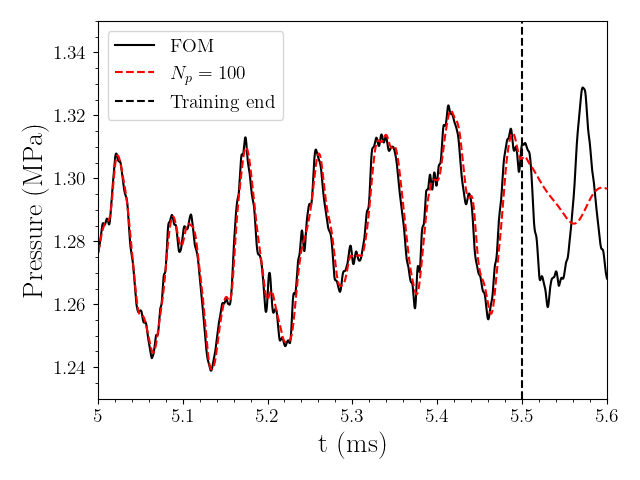
\includegraphics[width=0.99\linewidth]{Chapters/AdaptiveResults/Images/cvrc/pressure_probe_static_future.png}
        \caption{\label{fig:cvrcStaticFutureState}CVRC pressure probe, unsampled MP-LSVT, $\numPrimModes = 100$, $\dt = 5 \times \dtFOM$.}
    \end{minipage}
    \hspace{0.5em}
    \begin{minipage}{0.45\linewidth}
        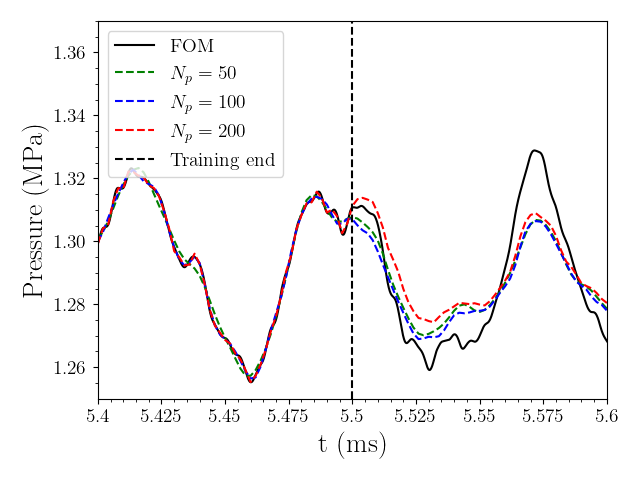
\includegraphics[width=0.99\linewidth]{Chapters/AdaptiveResults/Images/cvrc/pressure_probe_projection.png}
        \caption{\label{fig:cvrcStaticProjProbe}CVRC pressure probe, projected solution, various $\numPrimModes$.}
    \end{minipage}
\end{figure}

This is made readily apparent by observing the average projection error over time in Fig.~\ref{fig:cvrcStaticProjTime}. After $\timeVar = 5.5$ ms, the projection error drastically increases, and increasing the dimension of the trial basis is unable to improve this at all. This can be visually observed in pressure probe measurements of the projected solution in Fig.~\ref{fig:cvrcStaticProjProbe}, where large discrepancies can be observed beyond $\timeVar = 5.6$ ms. Further, comparisons of the FOM and projected pressure and temperature fields at $\timeVar = 5.6$ ms can be seen in Figs.~\ref{fig:cvrcStaticPressureProjSlice} and~\ref{fig:cvrcStaticTempProjSlice}. In both instances, the solution appears smeared and more axisymmetric, lacking most of the transient features of the flow field such as the  highly distorted flame front in the combustion chamber.

\begin{figure}
    \centering
    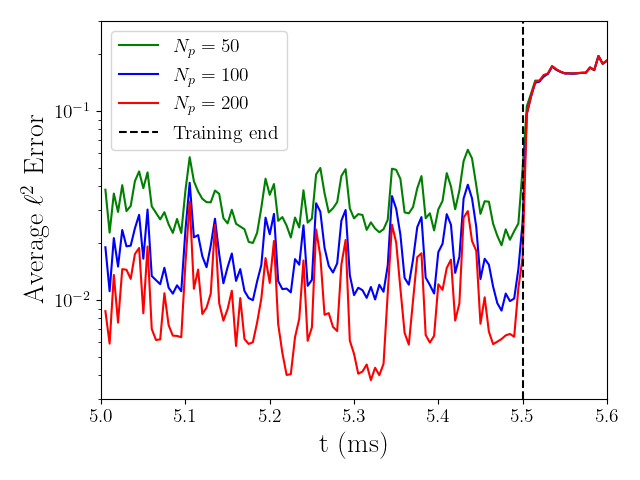
\includegraphics[width=0.75\linewidth]{Chapters/AdaptiveResults/Images/cvrc/proj_err_time.png}
    \caption{\label{fig:cvrcStaticProjTime}CVRC average projection error over time, various $\numPrimModes$.}
\end{figure}

\begin{figure}
	\begin{minipage}{0.99\linewidth}
		\raisebox{-0.5\height}{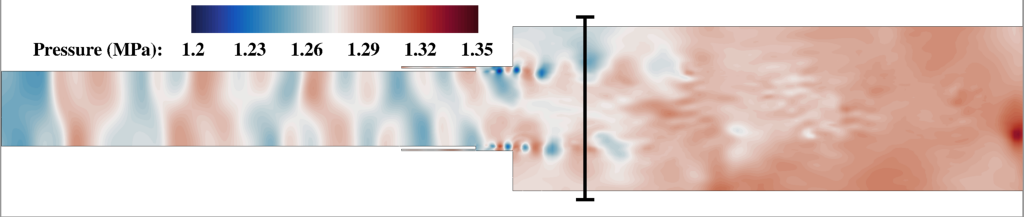
\includegraphics[width=0.84\linewidth,trim={0.5em 0.5em 0.5em 0.5em},clip]{Chapters/AdaptiveResults/Images/cvrc/fieldContours/fom_pressure_z.png}}
		\raisebox{-0.5\height}{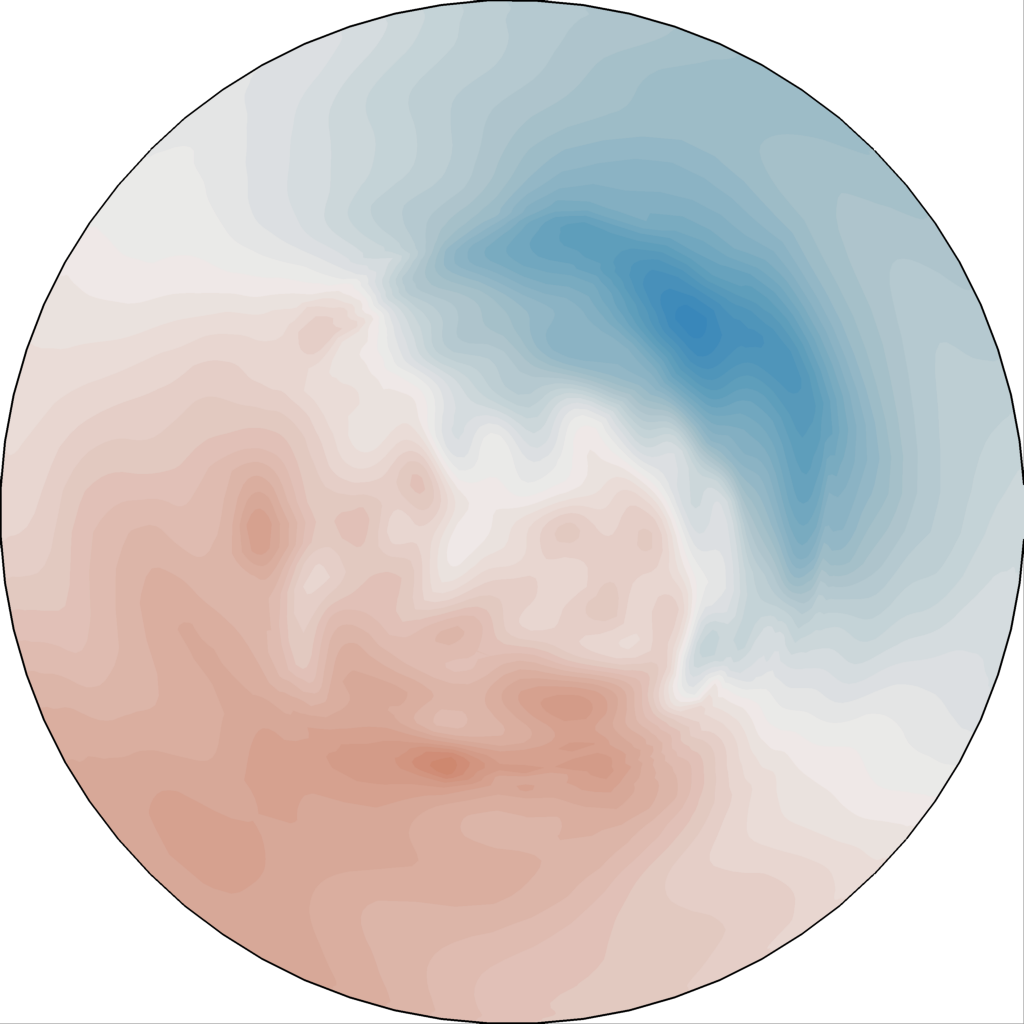
\includegraphics[width=0.14\linewidth,trim={0.0em 0.1em 0.0em 0.1em},clip]{Chapters/AdaptiveResults/Images/cvrc/fieldContours/fom_pressure_x.png}}
	\end{minipage}
    \begin{minipage}{0.99\linewidth}
		\raisebox{-0.5\height}{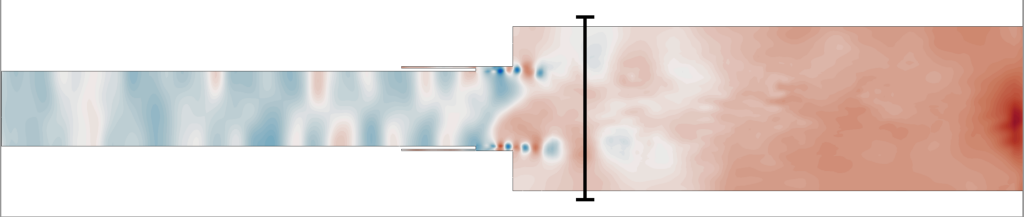
\includegraphics[width=0.84\linewidth,trim={0.5em 0.5em 0.5em 0.5em},clip]{Chapters/AdaptiveResults/Images/cvrc/fieldContours/proj_pressure_z.png}}
		\raisebox{-0.5\height}{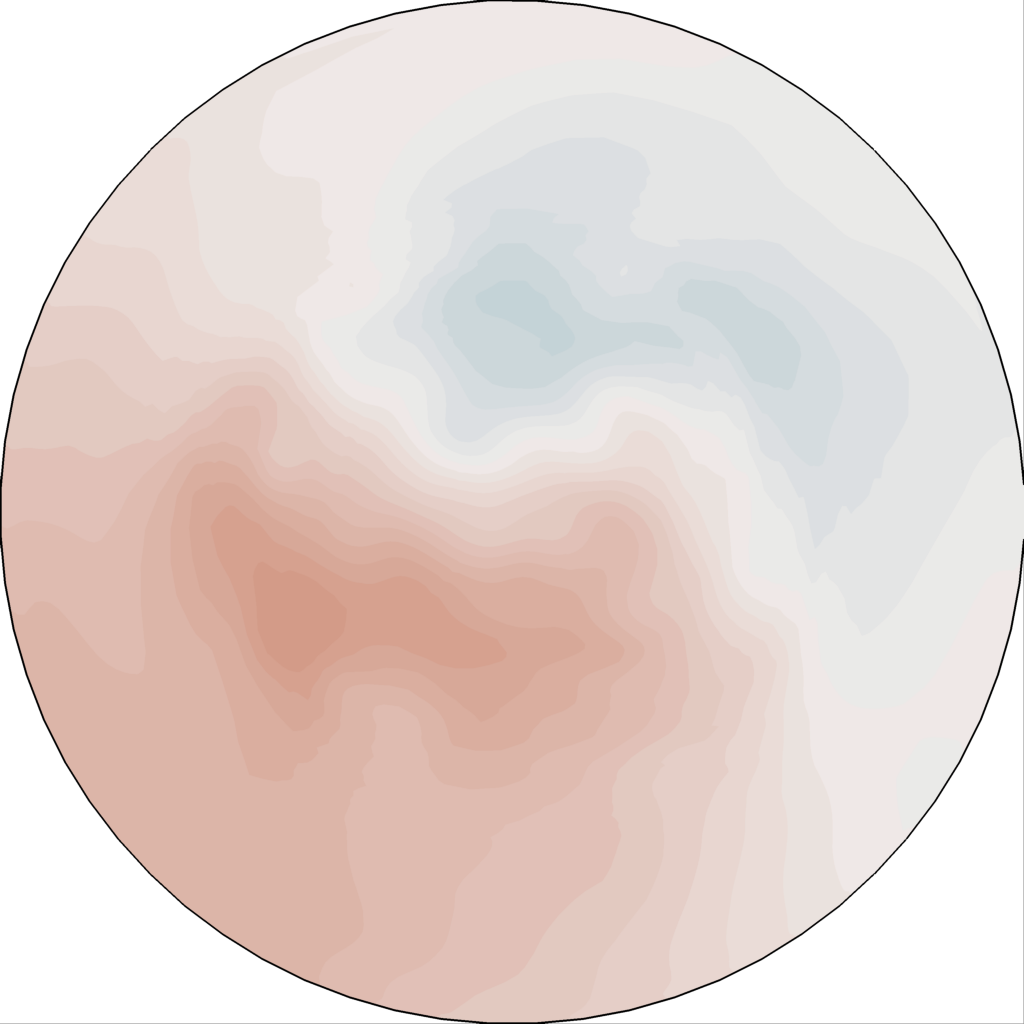
\includegraphics[width=0.14\linewidth,trim={0.0em 0.1em 0.0em 0.1em},clip]{Chapters/AdaptiveResults/Images/cvrc/fieldContours/proj_pressure_x.png}}
	\end{minipage}
    \caption{\label{fig:cvrcStaticPressureProjSlice}CVRC pressure field beyond training bounds, $\timeVar = 5.6$ ms, FOM at top and projected solution for $\numPrimModes = 100$ below.}
\end{figure}

\begin{figure}
	\begin{minipage}{0.99\linewidth}
		\raisebox{-0.5\height}{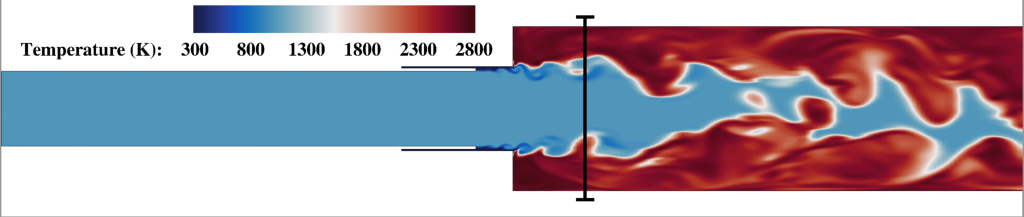
\includegraphics[width=0.84\linewidth,trim={0.5em 0.5em 0.5em 0.5em},clip]{Chapters/AdaptiveResults/Images/cvrc/fieldContours/fom_temperature_z.png}}
		\raisebox{-0.5\height}{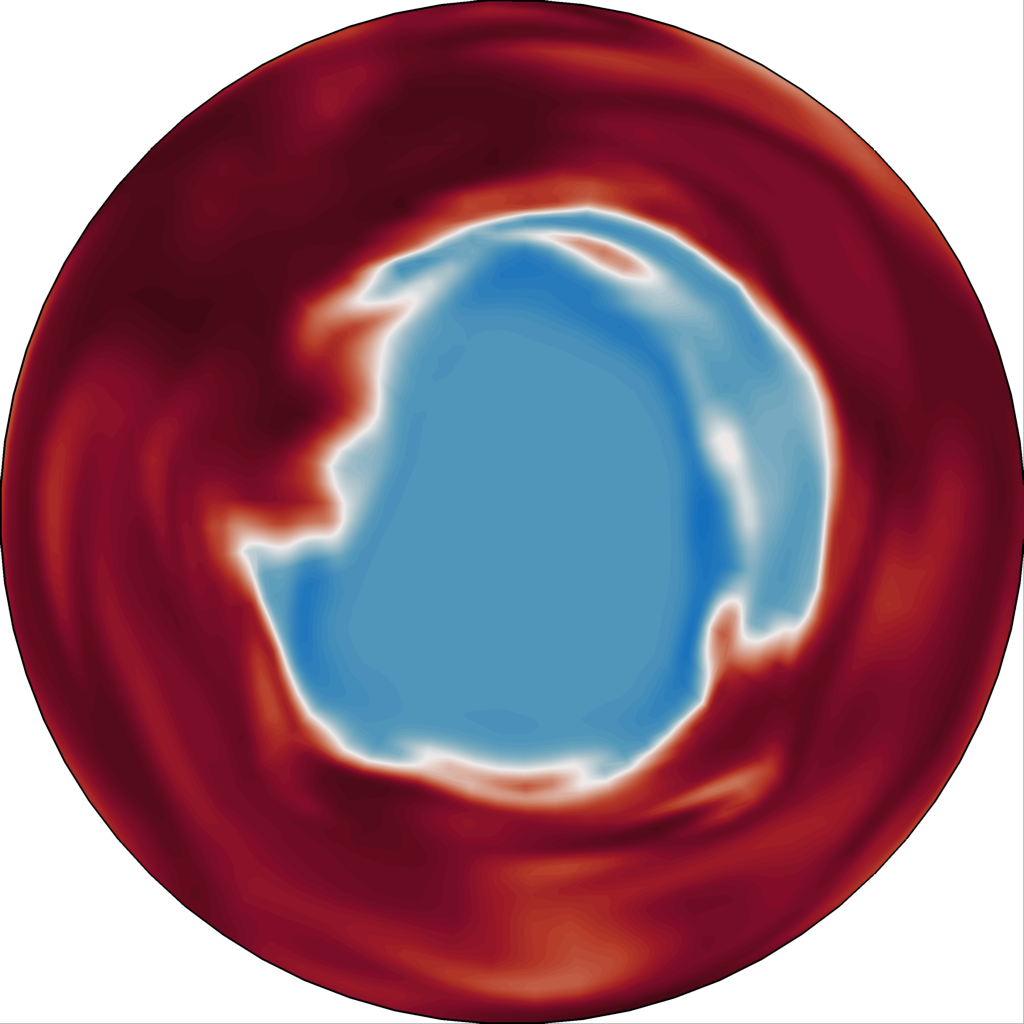
\includegraphics[width=0.14\linewidth,trim={0.0em 0.1em 0.0em 0.1em},clip]{Chapters/AdaptiveResults/Images/cvrc/fieldContours/fom_temperature_x.png}}
	\end{minipage}
    \begin{minipage}{0.99\linewidth}
		\raisebox{-0.5\height}{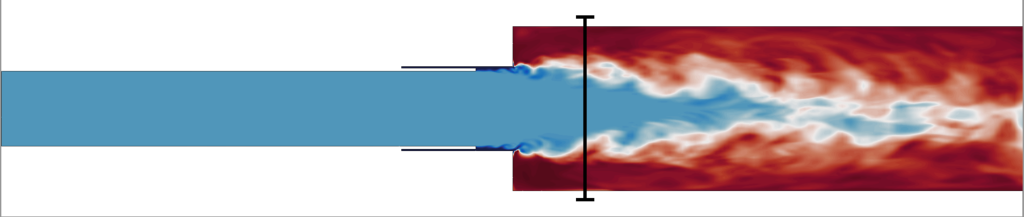
\includegraphics[width=0.84\linewidth,trim={0.5em 0.5em 0.5em 0.5em},clip]{Chapters/AdaptiveResults/Images/cvrc/fieldContours/proj_temperature_z.png}}
		\raisebox{-0.5\height}{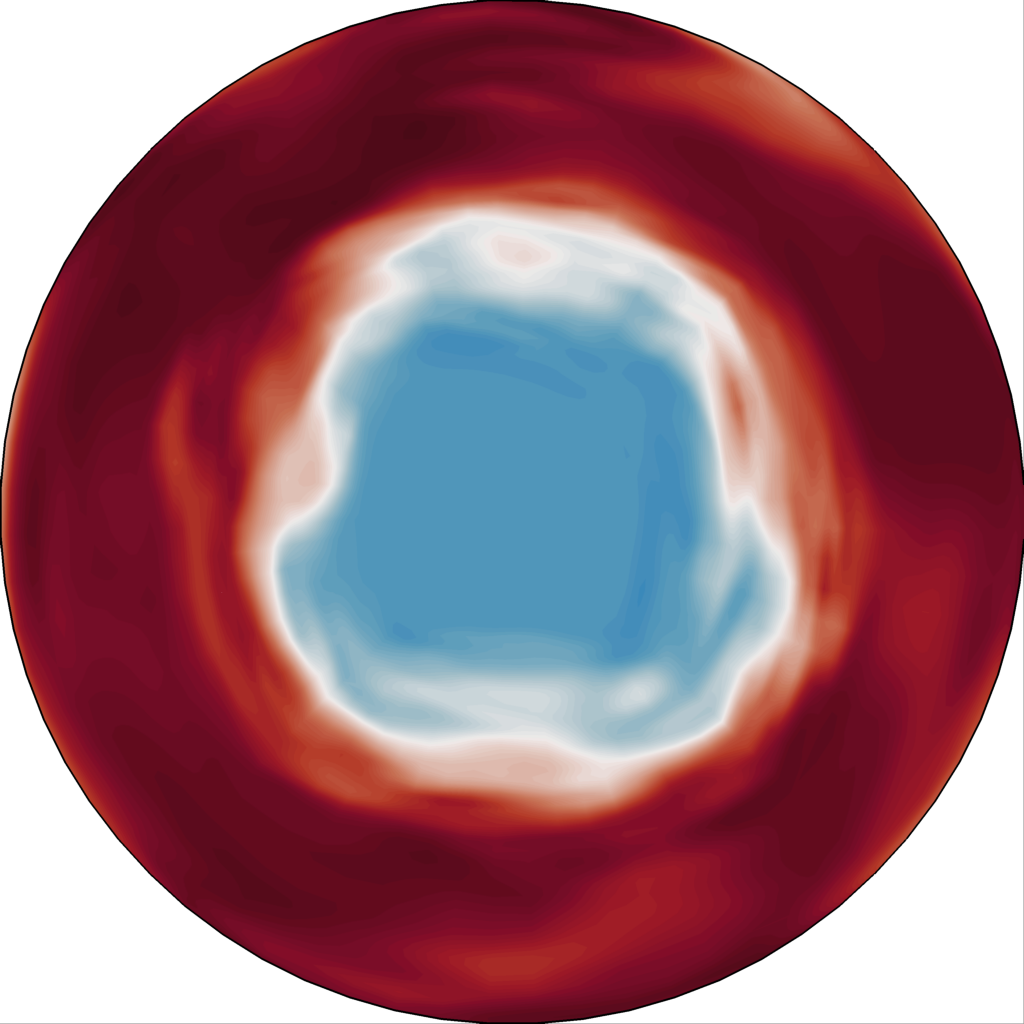
\includegraphics[width=0.14\linewidth,trim={0.0em 0.1em 0.0em 0.1em},clip]{Chapters/AdaptiveResults/Images/cvrc/fieldContours/proj_temperature_x.png}}
	\end{minipage}
    \caption{\label{fig:cvrcStaticTempProjSlice}CVRC temperture field beyond training bounds, $\timeVar = 5.6$ ms, FOM at top and projected solution for $\numPrimModes = 100$ below.}
\end{figure}

As discussed in Section~\ref{sec:adaptation}, adaptation of the trial basis during the online PROM runtime proposes a solution to this lack of trial space expressiveness. To achieve computational speedup, adaptation of the HPROM sample mesh has also been explored. In the following section, one approach for online HPROM adaptation is investigated. 